\documentclass{article}

\usepackage{graphicx}
\usepackage{amsmath}
\usepackage{amsthm}
\usepackage{amssymb}
\usepackage{fancyhdr}
\usepackage{hyperref}
\usepackage[dvipsnames]{xcolor}
\usepackage{enumitem}
\usepackage{minted}
%%%%% NEW MATH DEFINITIONS %%%%%

\usepackage{amsmath,amsfonts,bm,bbm}

\def\ind{{\mathbbm{1}}}

% Mark sections of captions for referring to divisions of figures
\newcommand{\figleft}{{\em (Left)}}
\newcommand{\figcenter}{{\em (Center)}}
\newcommand{\figright}{{\em (Right)}}
\newcommand{\figtop}{{\em (Top)}}
\newcommand{\figbottom}{{\em (Bottom)}}
\newcommand{\captiona}{{\em (a)}}
\newcommand{\captionb}{{\em (b)}}
\newcommand{\captionc}{{\em (c)}}
\newcommand{\captiond}{{\em (d)}}
\newcommand{\figleftt}{{\em Left}}
\newcommand{\figcentert}{{\em Center}}
\newcommand{\figrightt}{{\em Right}}
\newcommand{\figtopt}{{\em Top}}
\newcommand{\figbottomt}{{\em Bottom}}
\newcommand{\captionat}{{\em a}}
\newcommand{\captionbt}{{\em b}}
\newcommand{\captionct}{{\em c}}
\newcommand{\captiondt}{{\em d}}

% Highlight a newly defined term
\newcommand{\newterm}[1]{{\bf #1}}


% Figure reference, lower-case.
\def\figref#1{figure~\ref{#1}}
% Figure reference, capital. For start of sentence
\def\Figref#1{Figure~\ref{#1}}
\def\twofigref#1#2{figures \ref{#1} and \ref{#2}}
\def\quadfigref#1#2#3#4{figures \ref{#1}, \ref{#2}, \ref{#3} and \ref{#4}}
% Section reference, lower-case.
\def\secref#1{section~\ref{#1}}
% Section reference, capital.
\def\Secref#1{Section~\ref{#1}}
% Reference to two sections.
\def\twosecrefs#1#2{sections \ref{#1} and \ref{#2}}
% Reference to three sections.
\def\secrefs#1#2#3{sections \ref{#1}, \ref{#2} and \ref{#3}}

\def\chapref#1{chapter~\ref{#1}}
% Reference to an equation, upper case.
\def\Chapref#1{Chapter~\ref{#1}}
% Reference to a range of chapters
\def\rangechapref#1#2{chapters\ref{#1}--\ref{#2}}
% Reference to an algorithm, lower-case.
\def\algref#1{algorithm~\ref{#1}}
% Reference to an algorithm, upper case.
\def\Algref#1{Algorithm~\ref{#1}}
\def\twoalgref#1#2{algorithms \ref{#1} and \ref{#2}}
\def\Twoalgref#1#2{Algorithms \ref{#1} and \ref{#2}}
% Reference to a part, lower case
\def\partref#1{part~\ref{#1}}
% Reference to a part, upper case
\def\Partref#1{Part~\ref{#1}}
\def\twopartref#1#2{parts \ref{#1} and \ref{#2}}

\def\ceil#1{\lceil #1 \rceil}
\def\floor#1{\lfloor #1 \rfloor}
\def\1{\bm{1}}
\newcommand{\train}{\mathcal{D}}
\newcommand{\valid}{\mathcal{D_{\mathrm{valid}}}}
\newcommand{\test}{\mathcal{D_{\mathrm{test}}}}

\def\eps{{\epsilon}}


% Random variables
\def\reta{{\textnormal{$\eta$}}}
\def\ra{{\textnormal{a}}}
\def\rb{{\textnormal{b}}}
\def\rc{{\textnormal{c}}}
\def\rd{{\textnormal{d}}}
\def\re{{\textnormal{e}}}
\def\rf{{\textnormal{f}}}
\def\rg{{\textnormal{g}}}
\def\rh{{\textnormal{h}}}
\def\ri{{\textnormal{i}}}
\def\rj{{\textnormal{j}}}
\def\rk{{\textnormal{k}}}
\def\rl{{\textnormal{l}}}
% rm is already a command, just don't name any random variables m
\def\rn{{\textnormal{n}}}
\def\ro{{\textnormal{o}}}
\def\rp{{\textnormal{p}}}
\def\rq{{\textnormal{q}}}
\def\rr{{\textnormal{r}}}
\def\rs{{\textnormal{s}}}
\def\rt{{\textnormal{t}}}
\def\ru{{\textnormal{u}}}
\def\rv{{\textnormal{v}}}
\def\rw{{\textnormal{w}}}
\def\rx{{\textnormal{x}}}
\def\ry{{\textnormal{y}}}
\def\rz{{\textnormal{z}}}

% Random vectors
\def\rvepsilon{{\mathbf{\epsilon}}}
\def\rvtheta{{\mathbf{\theta}}}
\def\rva{{\mathbf{a}}}
\def\rvb{{\mathbf{b}}}
\def\rvc{{\mathbf{c}}}
\def\rvd{{\mathbf{d}}}
\def\rve{{\mathbf{e}}}
\def\rvf{{\mathbf{f}}}
\def\rvg{{\mathbf{g}}}
\def\rvh{{\mathbf{h}}}
\def\rvu{{\mathbf{i}}}
\def\rvj{{\mathbf{j}}}
\def\rvk{{\mathbf{k}}}
\def\rvl{{\mathbf{l}}}
\def\rvm{{\mathbf{m}}}
\def\rvn{{\mathbf{n}}}
\def\rvo{{\mathbf{o}}}
\def\rvp{{\mathbf{p}}}
\def\rvq{{\mathbf{q}}}
\def\rvr{{\mathbf{r}}}
\def\rvs{{\mathbf{s}}}
\def\rvt{{\mathbf{t}}}
\def\rvu{{\mathbf{u}}}
\def\rvv{{\mathbf{v}}}
\def\rvw{{\mathbf{w}}}
\def\rvx{{\mathbf{x}}}
\def\rvy{{\mathbf{y}}}
\def\rvz{{\mathbf{z}}}

% Elements of random vectors
\def\erva{{\textnormal{a}}}
\def\ervb{{\textnormal{b}}}
\def\ervc{{\textnormal{c}}}
\def\ervd{{\textnormal{d}}}
\def\erve{{\textnormal{e}}}
\def\ervf{{\textnormal{f}}}
\def\ervg{{\textnormal{g}}}
\def\ervh{{\textnormal{h}}}
\def\ervi{{\textnormal{i}}}
\def\ervj{{\textnormal{j}}}
\def\ervk{{\textnormal{k}}}
\def\ervl{{\textnormal{l}}}
\def\ervm{{\textnormal{m}}}
\def\ervn{{\textnormal{n}}}
\def\ervo{{\textnormal{o}}}
\def\ervp{{\textnormal{p}}}
\def\ervq{{\textnormal{q}}}
\def\ervr{{\textnormal{r}}}
\def\ervs{{\textnormal{s}}}
\def\ervt{{\textnormal{t}}}
\def\ervu{{\textnormal{u}}}
\def\ervv{{\textnormal{v}}}
\def\ervw{{\textnormal{w}}}
\def\ervx{{\textnormal{x}}}
\def\ervy{{\textnormal{y}}}
\def\ervz{{\textnormal{z}}}

% Random matrices
\def\rmA{{\mathbf{A}}}
\def\rmB{{\mathbf{B}}}
\def\rmC{{\mathbf{C}}}
\def\rmD{{\mathbf{D}}}
\def\rmE{{\mathbf{E}}}
\def\rmF{{\mathbf{F}}}
\def\rmG{{\mathbf{G}}}
\def\rmH{{\mathbf{H}}}
\def\rmI{{\mathbf{I}}}
\def\rmJ{{\mathbf{J}}}
\def\rmK{{\mathbf{K}}}
\def\rmL{{\mathbf{L}}}
\def\rmM{{\mathbf{M}}}
\def\rmN{{\mathbf{N}}}
\def\rmO{{\mathbf{O}}}
\def\rmP{{\mathbf{P}}}
\def\rmQ{{\mathbf{Q}}}
\def\rmR{{\mathbf{R}}}
\def\rmS{{\mathbf{S}}}
\def\rmT{{\mathbf{T}}}
\def\rmU{{\mathbf{U}}}
\def\rmV{{\mathbf{V}}}
\def\rmW{{\mathbf{W}}}
\def\rmX{{\mathbf{X}}}
\def\rmY{{\mathbf{Y}}}
\def\rmZ{{\mathbf{Z}}}
\def\rmtheta{{\mathbf{\Theta}}}
% Elements of random matrices
\def\ermA{{\textnormal{A}}}
\def\ermB{{\textnormal{B}}}
\def\ermC{{\textnormal{C}}}
\def\ermD{{\textnormal{D}}}
\def\ermE{{\textnormal{E}}}
\def\ermF{{\textnormal{F}}}
\def\ermG{{\textnormal{G}}}
\def\ermH{{\textnormal{H}}}
\def\ermI{{\textnormal{I}}}
\def\ermJ{{\textnormal{J}}}
\def\ermK{{\textnormal{K}}}
\def\ermL{{\textnormal{L}}}
\def\ermM{{\textnormal{M}}}
\def\ermN{{\textnormal{N}}}
\def\ermO{{\textnormal{O}}}
\def\ermP{{\textnormal{P}}}
\def\ermQ{{\textnormal{Q}}}
\def\ermR{{\textnormal{R}}}
\def\ermS{{\textnormal{S}}}
\def\ermT{{\textnormal{T}}}
\def\ermU{{\textnormal{U}}}
\def\ermV{{\textnormal{V}}}
\def\ermW{{\textnormal{W}}}
\def\ermX{{\textnormal{X}}}
\def\ermY{{\textnormal{Y}}}
\def\ermZ{{\textnormal{Z}}}

% Vectors
\def\vzero{{\bm{0}}}
\def\vone{{\bm{1}}}
\def\vmu{{\bm{\mu}}}
\def\vtheta{{\bm{\theta}}}
\def\va{{\bm{a}}}
\def\vb{{\bm{b}}}
\def\vc{{\bm{c}}}
\def\vd{{\bm{d}}}
\def\ve{{\bm{e}}}
\def\vf{{\bm{f}}}
\def\vg{{\bm{g}}}
\def\vh{{\bm{h}}}
\def\vi{{\bm{i}}}
\def\vj{{\bm{j}}}
\def\vk{{\bm{k}}}
\def\vl{{\bm{l}}}
\def\vm{{\bm{m}}}
\def\vn{{\bm{n}}}
\def\vo{{\bm{o}}}
\def\vp{{\bm{p}}}
\def\vq{{\bm{q}}}
\def\vr{{\bm{r}}}
\def\vs{{\bm{s}}}
\def\vt{{\bm{t}}}
\def\vu{{\bm{u}}}
\def\vv{{\bm{v}}}
\def\vw{{\bm{w}}}
\def\vx{{\bm{x}}}
\def\vy{{\bm{y}}}
\def\vz{{\bm{z}}}

% Elements of vectors
\def\evalpha{{\alpha}}
\def\evbeta{{\beta}}
\def\evepsilon{{\epsilon}}
\def\evlambda{{\lambda}}
\def\evomega{{\omega}}
\def\evmu{{\mu}}
\def\evpsi{{\psi}}
\def\evsigma{{\sigma}}
\def\evtheta{{\theta}}
\def\eva{{a}}
\def\evb{{b}}
\def\evc{{c}}
\def\evd{{d}}
\def\eve{{e}}
\def\evf{{f}}
\def\evg{{g}}
\def\evh{{h}}
\def\evi{{i}}
\def\evj{{j}}
\def\evk{{k}}
\def\evl{{l}}
\def\evm{{m}}
\def\evn{{n}}
\def\evo{{o}}
\def\evp{{p}}
\def\evq{{q}}
\def\evr{{r}}
\def\evs{{s}}
\def\evt{{t}}
\def\evu{{u}}
\def\evv{{v}}
\def\evw{{w}}
\def\evx{{x}}
\def\evy{{y}}
\def\evz{{z}}

% Matrix
\def\mA{{\bm{A}}}
\def\mB{{\bm{B}}}
\def\mC{{\bm{C}}}
\def\mD{{\bm{D}}}
\def\mE{{\bm{E}}}
\def\mF{{\bm{F}}}
\def\mG{{\bm{G}}}
\def\mH{{\bm{H}}}
\def\mI{{\bm{I}}}
\def\mJ{{\bm{J}}}
\def\mK{{\bm{K}}}
\def\mL{{\bm{L}}}
\def\mM{{\bm{M}}}
\def\mN{{\bm{N}}}
\def\mO{{\bm{O}}}
\def\mP{{\bm{P}}}
\def\mQ{{\bm{Q}}}
\def\mR{{\bm{R}}}
\def\mS{{\bm{S}}}
\def\mT{{\bm{T}}}
\def\mU{{\bm{U}}}
\def\mV{{\bm{V}}}
\def\mW{{\bm{W}}}
\def\mX{{\bm{X}}}
\def\mY{{\bm{Y}}}
\def\mZ{{\bm{Z}}}
\def\mBeta{{\bm{\beta}}}
\def\mPhi{{\bm{\Phi}}}
\def\mLambda{{\bm{\Lambda}}}
\def\mSigma{{\bm{\Sigma}}}

% Tensor
\DeclareMathAlphabet{\mathsfit}{\encodingdefault}{\sfdefault}{m}{sl}
\SetMathAlphabet{\mathsfit}{bold}{\encodingdefault}{\sfdefault}{bx}{n}
\newcommand{\tens}[1]{\bm{\mathsfit{#1}}}
\def\tA{{\tens{A}}}
\def\tB{{\tens{B}}}
\def\tC{{\tens{C}}}
\def\tD{{\tens{D}}}
\def\tE{{\tens{E}}}
\def\tF{{\tens{F}}}
\def\tG{{\tens{G}}}
\def\tH{{\tens{H}}}
\def\tI{{\tens{I}}}
\def\tJ{{\tens{J}}}
\def\tK{{\tens{K}}}
\def\tL{{\tens{L}}}
\def\tM{{\tens{M}}}
\def\tN{{\tens{N}}}
\def\tO{{\tens{O}}}
\def\tP{{\tens{P}}}
\def\tQ{{\tens{Q}}}
\def\tR{{\tens{R}}}
\def\tS{{\tens{S}}}
\def\tT{{\tens{T}}}
\def\tU{{\tens{U}}}
\def\tV{{\tens{V}}}
\def\tW{{\tens{W}}}
\def\tX{{\tens{X}}}
\def\tY{{\tens{Y}}}
\def\tZ{{\tens{Z}}}


% Graph
\def\gA{{\mathcal{A}}}
\def\gB{{\mathcal{B}}}
\def\gC{{\mathcal{C}}}
\def\gD{{\mathcal{D}}}
\def\gE{{\mathcal{E}}}
\def\gF{{\mathcal{F}}}
\def\gG{{\mathcal{G}}}
\def\gH{{\mathcal{H}}}
\def\gI{{\mathcal{I}}}
\def\gJ{{\mathcal{J}}}
\def\gK{{\mathcal{K}}}
\def\gL{{\mathcal{L}}}
\def\gM{{\mathcal{M}}}
\def\gN{{\mathcal{N}}}
\def\gO{{\mathcal{O}}}
\def\gP{{\mathcal{P}}}
\def\gQ{{\mathcal{Q}}}
\def\gR{{\mathcal{R}}}
\def\gS{{\mathcal{S}}}
\def\gT{{\mathcal{T}}}
\def\gU{{\mathcal{U}}}
\def\gV{{\mathcal{V}}}
\def\gW{{\mathcal{W}}}
\def\gX{{\mathcal{X}}}
\def\gY{{\mathcal{Y}}}
\def\gZ{{\mathcal{Z}}}

% Sets
\def\sA{{\mathbb{A}}}
\def\sB{{\mathbb{B}}}
\def\sC{{\mathbb{C}}}
\def\sD{{\mathbb{D}}}
% Don't use a set called E, because this would be the same as our symbol
% for expectation.
\def\sF{{\mathbb{F}}}
\def\sG{{\mathbb{G}}}
\def\sH{{\mathbb{H}}}
\def\sI{{\mathbb{I}}}
\def\sJ{{\mathbb{J}}}
\def\sK{{\mathbb{K}}}
\def\sL{{\mathbb{L}}}
\def\sM{{\mathbb{M}}}
\def\sN{{\mathbb{N}}}
\def\sO{{\mathbb{O}}}
\def\sP{{\mathbb{P}}}
\def\sQ{{\mathbb{Q}}}
\def\sR{{\mathbb{R}}}
\def\sS{{\mathbb{S}}}
\def\sT{{\mathbb{T}}}
\def\sU{{\mathbb{U}}}
\def\sV{{\mathbb{V}}}
\def\sW{{\mathbb{W}}}
\def\sX{{\mathbb{X}}}
\def\sY{{\mathbb{Y}}}
\def\sZ{{\mathbb{Z}}}

% Entries of a matrix
\def\emLambda{{\Lambda}}
\def\emA{{A}}
\def\emB{{B}}
\def\emC{{C}}
\def\emD{{D}}
\def\emE{{E}}
\def\emF{{F}}
\def\emG{{G}}
\def\emH{{H}}
\def\emI{{I}}
\def\emJ{{J}}
\def\emK{{K}}
\def\emL{{L}}
\def\emM{{M}}
\def\emN{{N}}
\def\emO{{O}}
\def\emP{{P}}
\def\emQ{{Q}}
\def\emR{{R}}
\def\emS{{S}}
\def\emT{{T}}
\def\emU{{U}}
\def\emV{{V}}
\def\emW{{W}}
\def\emX{{X}}
\def\emY{{Y}}
\def\emZ{{Z}}
\def\emSigma{{\Sigma}}

% entries of a tensor
% Same font as tensor, without \bm wrapper
\newcommand{\etens}[1]{\mathsfit{#1}}
\def\etLambda{{\etens{\Lambda}}}
\def\etA{{\etens{A}}}
\def\etB{{\etens{B}}}
\def\etC{{\etens{C}}}
\def\etD{{\etens{D}}}
\def\etE{{\etens{E}}}
\def\etF{{\etens{F}}}
\def\etG{{\etens{G}}}
\def\etH{{\etens{H}}}
\def\etI{{\etens{I}}}
\def\etJ{{\etens{J}}}
\def\etK{{\etens{K}}}
\def\etL{{\etens{L}}}
\def\etM{{\etens{M}}}
\def\etN{{\etens{N}}}
\def\etO{{\etens{O}}}
\def\etP{{\etens{P}}}
\def\etQ{{\etens{Q}}}
\def\etR{{\etens{R}}}
\def\etS{{\etens{S}}}
\def\etT{{\etens{T}}}
\def\etU{{\etens{U}}}
\def\etV{{\etens{V}}}
\def\etW{{\etens{W}}}
\def\etX{{\etens{X}}}
\def\etY{{\etens{Y}}}
\def\etZ{{\etens{Z}}}


\DeclareMathOperator{\E}{\mathbb{E}}
\newcommand{\Ls}{\mathcal{L}}
\newcommand{\R}{\mathbb{R}}
\newcommand{\emp}{\tilde{p}}
\newcommand{\lr}{\alpha}
\newcommand{\reg}{\lambda}
\newcommand{\sigmoid}{\sigma}
\newcommand{\softplus}{\zeta}
\newcommand{\KL}{D_{\mathrm{KL}}}
\newcommand{\Var}{\mathrm{Var}}
\newcommand{\standarderror}{\mathrm{SE}}
\newcommand{\Cov}{\mathrm{Cov}}
\DeclareMathOperator*{\argmax}{arg\,max}
\DeclareMathOperator*{\argmin}{arg\,min}

\DeclareMathOperator{\sign}{sign}
\DeclareMathOperator{\Tr}{Tr}
\let\ab\allowbreak

\newcommand{\vbar}[1]{\bigg\rvert_{#1}}
\newcommand\at[2]{\left.#1\right|_{#2}}
\newcommand{\bs}[1]{\boldsymbol{#1}}

\newcommand{\sigx}[1]{\sigma_{x,#1}}
\newcommand{\sigb}[1]{\sigma_{\beta,#1}}

\newcommand{\dd}{\mathrm{d}} %for integration

\newcommand{\wipcom}[1]{\textcolor{red}{WIP: #1}}
\newcommand{\sol}[1]{\textcolor{gray}{}}
\newcommand{\nyuparagraph}[1]{\vspace{0.3cm}\textcolor{nyupurple}{\bf \large #1}\\}
\newcommand{\code}[1]{\texttt{#1}}
\newcommand{\nll}{\rm NLL}

\pagestyle{empty} \addtolength{\textwidth}{1.0in}
\addtolength{\textheight}{0.5in} \addtolength{\oddsidemargin}{-0.5in}
\addtolength{\evensidemargin}{0.5in}
\newcommand{\ruleskip}{\bigskip\hrule\bigskip}
\newcommand{\nodify}[1]{{\sc #1}} \newcommand{\points}[1]{{\textbf{[#1
points]}}}

\newcommand{\bitem}{\begin{list}{$\bullet$}%
{\setlength{\itemsep}{0pt}\setlength{\topsep}{0pt}%
\setlength{\rightmargin}{0pt}}} \newcommand{\eitem}{\end{list}}

\definecolor{nyupurple}{RGB}{134, 0, 179}
\setlength{\parindent}{0pt} \setlength{\parskip}{0.5ex}

\DeclareUnicodeCharacter{2212}{-}

\theoremstyle{plain}
\newtheorem*{thm*}{\protect\theoremname}
\theoremstyle{definition}
\newtheorem*{defn*}{\protect\definitionname}

\begin{document}
\newcounter{saveenum}

\pagestyle{myheadings} \markboth{}{\color{nyupurple} DS-GA-1003 - Spring 2023}

\begin{center}
{\Large
Homework 4: Probabilistic models
} 
\end{center}

{
{ \color{nyupurple} \textbf{Due:} Wednesday, March 22, 2023 at 11:59PM EST} 
} 

\textbf{Instructions: }Your answers to the questions below, including plots and mathematical work, should be submitted as a single PDF file.  It's preferred that you write your answers using software that typesets mathematics (e.g.LaTeX, LyX, or MathJax via iPython), though if you need to you may scan handwritten work.  You may find the \href{https://github.com/gpoore/minted}{minted} package convenient for including source code in your LaTeX document.  If you are using LyX, then the \href{https://en.wikibooks.org/wiki/LaTeX/Source_Code_Listings}{listings} package tends to work better.

\ruleskip

\section{Logistic Regression}
\label{sec:lr}
Consider a binary classification setting with input
space $\mathcal{X}=\mathbb{R}^{d}$, outcome space $\mathcal{Y}_{\pm}=\left\{ -1,1\right\} $,
and a dataset $\mathcal{D}=\left((x^{(1)},y^{(1)}),\ldots,(x^{(n)},y^{(n)})\right)$.


\nyuparagraph{\label{subsec:erm-bernoulli-setup}Equivalence of ERM and probabilistic
approaches}
In the lecture we derived logistic regression using the Bernoulli response distribution.
In this problem you will show that it is equivalent to ERM with logistic loss.

\textbf{ERM with logistic loss.}\\
Consider a linear scoring function in the space $\mathcal{F}_{\text{score}}=\left\{ x\mapsto x^{T}w\mid w\in\mathbb{R}^{d}\right\} $.
A simple way to make predictions (similar to what we've seen with the perceptron algorithm)
is to predict $\hat{y}=1$ if $x^Tw > 0$, or $\hat{y} = \text{sign}(x^Tw)$.
Accordingly, we consider margin-based loss functions that relate the loss with the margin, $yx^Tw$.
A positive margin means that $x^Tw$ has the same sign as $y$, i.e. a correct prediction.
Specifically, let's consider the \textbf{logistic loss} function $\ell_{\text{logistic}}(y, w)=\log\left(1+\exp(-yw^Tx)\right)$.
This is a margin-based loss function that you have now encountered several times.
%  and an upper bound of the 0-1 loss.
Given the logistic loss, we can now minimize the empirical risk on our dataset $\mathcal{D}$ to obtain an estimate of the parameters, $\hat{w}$.

\textbf{MLE with a Bernoulli response distribution and the logistic link function.}\\
As discussed in the lecture, given that
$p(y=1 \mid x; w) = 1 / (1 + \exp(-x^Tw))$,
we can estimate $w$ by maximizing the likelihood, or equivalently,
minimizing the negative log-likelihood ($\nll_{\mathcal{D}}(w)$~in short) of the data.

\begin{enumerate}
  \setcounter{enumi}{\value{saveenum}}
  \item Show that the two approaches are equivalent, i.e. they will produce the same solution for $w$.
\setcounter{saveenum}{\value{enumi}}
\begin{itemize}
\color{blue}
\item first re-write the erm approach  
\begin{itemize}
    \item so recall that in ERM the empirical risk of a function is given by 
    \item $$\hat{R}_{n}=\frac{1}{n}\Sigma_{i=1}^{n}\ell(f(x^i),y^i)$$
    \item so in the case of logistic loss we can see that our optimal weight vector will be given by  $$\hat{w}_{erm}=argmin_{w\in \mathbb{R}^{d}}\frac{1}{n}\Sigma_{i=1}^{n}\ell_{log}(f(x^i),y^i)=argmin_{w\in \mathbb{R}^{d}}\frac{1}{n}\Sigma_{i=1}^{n}log(1+e^{-y^iw^tx^i})$$
    \item as shown in homework 2 question 26 this expression can be re-written as  $\hat{w}_{erm}=argmin_{w\in \mathbb{R}^{d}}\frac{1}{n}\Sigma_{i=1}^{n}\ell_{log}(f(x^i),y^i)=argmin_{w\in \mathbb{R}^{d}}\frac{1}{n}\Sigma_{i=1}^{n}log(1+e^{-y^iw^tx^i})=argmin_{w\in \mathbb{R}^{d}}\frac{1}{2n}\Sigma_{i=1}^{n}(1+y^i)log(1+e^{-w^tx^i})+(1-y^i)log(1+e^{w^tx^i})$
    \item further we know that maximising the inverse of a function is equiv lent to minimizing it.
    that is     $\hat{w}_{erm}=argmin_{w\in \mathbb{R}^{d}}\frac{1}{2n}\Sigma_{i=1}^{n}(1+y^i)log(1+e^{-w^tx^i})+(1-y^i)log(1+e^{w^tx^i})\iff argmax_{w\in \mathbb{R}^{d}}\frac{1}{2n}\Sigma_{i=1}^{n}(1+y^i)log(\frac{1}{log(1+e^{-w^tx^i})})+(1-y^i)\frac{1}{log(1+e^{w^tx^i})}) $
    \item and further as the log is a monotonic transformation we can say 
    $\hat{w}_{erm}=argmin_{w\in \mathbb{R}^{d}}\frac{1}{2n}\Sigma_{i=1}^{n}(1+y^i)log(1+e^{-w^tx^i})+(1-y^i)log(1+e^{w^tx^i})\iff \iff argmax_{w\in \mathbb{R}^{d}}\frac{1}{2n}\Sigma_{i=1}^{n}(1+y^i)log(\frac{1}{log(1+e^{-w^tx^i})})+(1-y^i)\frac{1}{log(1+e^{w^tx^i})})  \iff argmax_{w\in \mathbb{R}^{d}}\frac{1}{2n}\Sigma_{i=1}^{n}(1+y^i)log(\frac{1}{1+e^{-w^tx^i}})+(1-y^i)log(\frac{1}{1+e^{w^tx^i}}) $
    \item notice further that if we define the sigmoid function as $f(x)=\frac{1}{1+e^{-x}}$
    we can express our problem as $\hat{w}_{erm}= argmax_{w\in \mathbb{R}^{d}}\frac{1}{2n}\Sigma_{i=1}^{n}(1+y^i)log(\frac{1}{1+e^{-w^tx^i}})+(1-y^i)log(\frac{1}{1+e^{w^tx^i}}) = argmax_{w\in \mathbb{R}^{d}}\frac{1}{2n}\Sigma_{i=1}^{n}(1+y^i)f(w^tx^i)+(1-y^i)f(-w^tx^i)$
    \item further note the following equality $1-f(x)=1-\frac{1}{1+e^{-x}}=\frac{e^{-x}}{1+e^{-x}}=\frac{1}{1+e^x}=f(-x)$
    \item so substituting this back into our erm function yields our final result for erm $$\hat{w}_{erm}=argmax_{w\in \mathbb{R}^{d}}\frac{1}{2n}\Sigma_{i=1}^{n}(1+y^i)log(f(x))+(1-y^i)log(1-f(x))$$
\end{itemize}
\item now we can re-writ the maximum likelihood approach. 
\begin{itemize}
    \item if we assume that our data is iid, and that each individual example is a Bernoulli random viable we can write the likelihood of our data set as $\mathcal{L}(D)=P(y^1,y^2...y^n|x^1...x^n,,w)=P(y^1|x^1,w)P(y^2|y^1,x^1,x^2,w)...=\Pi_{i=1}^{n}P(y^i|x^i, w)$ 
    \item then our log likelihood of the data set is $\ell(d)=log(\mathcal{L}(D)=\Sigma_{i=1}^{n}P(y^i|x^i,w)$
    \item in the binary classification case with $y\in\{-1,1\}$this becomes $\ell(d)=\frac{1}{2}\Sigma_{i=1}^{n}(1+y^i)P(y^i=1|x^i,w)+(1-y^i)P(y^i=-1|x^i,w)$
    \item under the assumptions of logistic regression $P(y=1|x,w)=f(w^tx)$ where f as defined above is the sigmoid function thus we have $\ell(d)=\frac{1}{2}\Sigma_{i=1}^{n}(1+y^i)f(w^tx^n)+(1-y^i)(1-f(w^tx^n)$
    \item so the weight vector this would yield would be    $\hat{w}_{mle}= argmax_{w\in \mathbb{R}^{d}}\frac{1}{2}\Sigma_{i=1}^{n}(1+y^i)log(\frac{1}{1+e^{-w^tx^i}})+(1-y^i)log(\frac{1}{1+e^{w^tx^i}}) $
\end{itemize}
\item so it is clear that the $\hat{w}_{erm}$ and $\hat{w}_{mle}$ only differ by a constant factor of $\frac{1}{n}$ which will not effect the arg max and thus $\hat{w}_{erm}=\hat{w}_{mle}$
\item now we can solve for $\hat{w}=\hat{w}_{erm}=\hat{w}_{mle}$
\begin{itemize}
    \item given $$\hat{w}= argmax_{w\in \mathbb{R}^{d}}\frac{1}{2}\Sigma_{i=1}^{n}(1+y^i)log(\frac{1}{1+e^{-w^tx^i}})+(1-y^i)log(\frac{1}{1+e^{w^tx^i}}) $$
    \item we can find the gradient with respect to w as $\nabla_{w}(\hat{w})=\frac{1}{2}\Sigma_{i=1}^{n}[\frac{y^i+1}{f(w^tx^i)}-\frac{1-y^i}{f(w^tx^i}]\frac{\partial f(w^tx^i)}{\partial w}=\frac{1}{2}\Sigma_{i=1}^{n}[\frac{y^i+1}{f(w^tx^i)}-\frac{1-y^i}{f(w^tx^i}](f(w^tx^i)(1-f(w^tx^i))(x^i)=\frac{1}{2}\Sigma_{i=1}^{n}[\frac{(y^n+1)(1-f(w^tx^n)- f(w^tx^n)(1-y^n)}{f(w^tx^n)(1-f(w^tx^n)}](f(w^tx^n)(1-f(w^tx^n))x^i=\frac{1}{2}\Sigma_{i=1}^{n}[y^n+1-2f(w^tx^n)]=\Sigma_{i=1}^{n}[\frac{y^n+1}{2}-f(w^tx^n)]$
\end{itemize}

 \end{itemize} 
\end{enumerate}



\newpage
\nyuparagraph{Linearly Separable Data}
\label{sec:linear}
In this problem, we will investigate the behavior of MLE for logistic regression when the data is linearly separable.

\begin{enumerate}
  \setcounter{enumi}{\value{saveenum}}
\item Show that the decision boundary of logistic regression is given by $\left\{x\colon x^Tw=0\right\}$.
Note that the set will not change if we multiply the weights by some constant $c$.
\begin{itemize}
    \color{blue}
    \item our decision boundary is the set of points such that we are equally likely to predict either class 
    \item this can thus be expressed in terms of the log odds between the two classes $log\frac{P(y=1|x,w)}{P(y=-1|x,w)}=log(\frac{P(y=1|x,\theta)}{1-P(y=1|x,\theta)})=log(\frac{\frac{1}{1+e^{-w^tx}}} {1-\frac{1}{1+e^{w^tx}}})=log(\frac{\frac{1}{1+e^{-w^tx}}} {\frac{e^{-w^tx}}{1+e^{w^tx}}})=log(\frac{1}{e^{-w^tx}})=log(1)-log(e^{-w^tx})=0-(-w^txlog(e))=w^tx$
    \item and we know that our decision boundary is the space such that the odds between the two classes is 1, or in other words the log odds between the two classes are zero. we showed above that the $log\frac{P(y=1|x,w)}{P(y=-1|x,w)}=log(\frac{P(y=1|x,\theta)}{1-P(y=1|x,\theta)})=w^tx=x^tw$ setting this equal to zero we see that the decision boundary is given by $\{x:x^tw=0\}$ in other words it s a hyperplane that is perpendicular to our weight vector w.  
    
\end{itemize}

\item Suppose the data is linearly separable and by gradient descent/ascent we have reached a decision boundary defined by $\hat{w}$ where all examples are classified correctly. 
Show that we can always increase the likelihood of the data by multiplying a scalar $c$ on $\hat{w}$,
which means that MLE is not well-defined in this case.
{(Hint: You can show this by taking the derivative of $L(c\hat{w})$ with respect to $c$, where $L$ is the likelihood function.)}
\begin{itemize}

    \color{blue}
    \item first note that the likelihood of our data in this case is given by $\ell(D,w)=\frac{1}{2}\Sigma_{i=1}^{n}( (1+y^i)log(P(y^i=1|x_i=1,w)) +((1-y^i)log(P(y^i=-1|x_i=1,w)))=\frac{1}{2}\Sigma_{i=1}^{n}((1+y^i)log(f(w^tx^i))+(1-y^i)log(1-f(w^tx^i))$
    \item so we can write the likelihood of our data set and weight vector times some constant c as $\ell(D,cw)=\frac{1}{2}\Sigma_{i=1}^{n}((1+y^i)log(f(cw^tx^i))+(1-y^i)log(1-f(cw^tx^i))$
    \item taking the derivative with respect to c we see that $\frac{\partial \ell}{\partial c}=\frac{1}{2}\Sigma_{i=1}^{n}[\frac{y^i+1}{f(cw^tx^i)} +\frac{1-y^i}{1-f(cw^tx^i)}]f(cw^tx^i)(1-f(xw^tx^i))(w^tx^i)=\Sigma_{i=1}^{n}[\frac{y^n+1}{2}-f(cw^tx^i)]w^tx^i=\Sigma_{i=1}^{n}[\frac{y^n+1}{2}-\frac{1}{1+e^{-cw^tx^n}}]w^tx^i$
    \item first off as we know the data is lineally separable if $w$ is a separating hyperplane $w^tx>0$ will always holds when $y^{i}=1$ and $w^{t}x<0$ will always hold when $y=-1$ 
    \item this tells us that  $\frac{\partial \ell}{\partial c}=\Sigma_{i=1}^{n}[\frac{y^n+1}{2}-\frac{1}{1+e^{-cw^tx^n}}]w^tx^i$ will always be increasing in c. 
    \item so we can keep geometrically the same hyperplane but arbitrarily increase our likelihood of seeing the data by increasing the constant on it $c$ which multiples our weight vector w.  
\end{itemize}


\setcounter{saveenum}{\value{enumi}}
\end{enumerate}

\nyuparagraph{\label{subsec:Regularized-Logistic-Regression}Regularized Logistic
Regression}
As we've shown in above, when the data is linearly separable,
MLE for logistic regression may end up with weights with very large magnitudes. Such a function is prone to overfitting.
In this part, we will apply regularization to fix the problem.

The $\ell_2$ regularized
logistic regression objective function can be defined as
\begin{eqnarray*}
J_{\text{logistic}}(w) & = & \hat{R}_{n}(w)+\lambda\|w\|^{2}\\
 & = & \frac{1}{n}\sum_{i=1}^{n}\log\left(1+\exp\left(-y^{(i)}w^{T}x^{(i)}\right)\right)+\lambda\|w\|^{2}.
\end{eqnarray*}
 
\begin{enumerate}
  \setcounter{enumi}{\value{saveenum}}
\item Prove that the objective function $J_{\text{logistic}}(w)$ is convex.
You may use any facts mentioned in the \href{https://davidrosenberg.github.io/mlcourse/Notes/convex-optimization.pdf}{convex optimization notes}
\begin{itemize}
    \color{blue}
    \item first off we know that the sum of two convex functions are convex. 
    \item so let us define $J(w)=f(w)+g(w)$ and prove that both $f(W)$ and $g(w)$ are convex separately
    \item first lets look as $f(w)=\frac{1}{n}\Sigma_{i=1}^{n}log(1+e^{-y^iw^tx^i}))$
    \begin{itemize}
        \item working form inside out we know that $e^x$ is convex over $\mahtbb{R}$
        \item we know that the function h(x)=1 is convex thus $1+e^{-y^iw^tx^i}$ is convex. 
        \item then we know $1+e^{-y^iw^tx^i}\geq 1$ since clearly the the smallest value $e^{x}$ can take is 0 
        \item further as we know log(x) is convex over $\mathbb{R}>0$ it must be the case that $log(1+e^{-y^iw^tx^i}))$ is convex
        \item finally we know that scaling and summing convex functions makes them remain convex thus we have shown $f(w)=\frac{1}{n}\Sigma_{i=1}^{n}log(1+e^{-y^iw^tx^i}))$ is convex
    \end{itemize}
    \item next lets look at $g(w)=\lambda||w||^2$
    \begin{itemize}
        \item to show a function f is convex it must be the case that $\forall \theta\in [0,1] \forall x,y\in dom f$ we must have $f(\theta x +(1-\theta)y)\leq \theta(f(x))+(1-\theta)(f(y))$
        \item so consider and arbitrary $\theta \in [0,1] ,x,y\in $dom(f). 
        \item we can see that $g(\theta x + (1-\theat) y)=\lambda||\theta x+ (1-\theta)y||^2\leq \lambda (||\theta x||+ ||(1-\theta)y||^2 $ (by the triangle inequality) = $\lambda \theta ||x||^2+ \lambda (1-\theta)||y||^2=\theta g(x)+(1-\theta)g(y)$ proving that g(x) is indeed convex
    \end{itemize}
\end{itemize}
.

\item Complete the \texttt{f\_objective} function in the skeleton code,
which computes the objective function for $J_{\text{logistic}}(w)$.
(Hint: you may get numerical overflow when computing the exponential literally,
e.g. try $e^{1000}$ in Numpy.
Make sure to read about the
\href{https://blog.feedly.com/tricks-of-the-trade-logsumexp/}{log-sum-exp trick}
and use the numpy function
\textit{ \href{https://docs.scipy.org/doc/numpy/reference/generated/numpy.logaddexp.html}{logaddexp}
}
to get accurate calculations
and to prevent overflow.

\begin{itemize}
    \color{blue}
    \item first note that in the case of our data $y\in \{0,1\}$
    \item recall from part 1, that this approach (ie using ERM) will yield the same sollution as MLE 
    \item thus we can work with the MLE objective of the from $j(w)=\frac{-1}{m}\Sigma_{i=1}^{n}(y^i)log(\frac{1}{1+e^{-w^tx^i}})+(1-y^i)log(\frac{1}{1+e^{w^tx^i}})+\lambda ||w||^2$
    \item we can further simplify this objective$j(w)=\frac{-1}{m}\Sigma_{i=1}^{n}(y^i)log(\frac{1}{1+e^{-w^tx^i}})+(1-y^i)log(\frac{1}{1+e^{w^tx^i}})+\lambda ||w||^2=\frac{-1}{m}\Sigma_{i=1}^{n}(y^i)[log({1})-log({1+e^{-w^tx^i}})]+(1-y^i)[log(1)-log({1+e^{w^tx^i}}))+\lambda ||w||^2=\Sigma_{i=1}^{n}\lambda ||w||^2-(y^i)[log({1+e^{-w^tx^i}})]-(1-y^i)[log({1+e^{w^tx^i}})])=\Sigma_{i=1}^{n}\lambda ||w||^2-(y^i)[log({e^{0}+e^{-w^tx^i}})]-(1-y^i)[log({e^{0}+e^{w^tx^i}})])$
      \item \inputminted[firstline=17, lastline=32, breaklines=True]{python}{hw_4_code.py}
\end{itemize}

\item Complete the \texttt{fit\_logistic\_regression\_function} in the skeleton
code using the \texttt{minimize} function from \texttt{scipy.optimize}.
Use this function to train
a model on the provided data. Make sure to take the appropriate preprocessing
steps, such as standardizing the data and adding a column for the
bias term. 
\begin{itemize}
    \
\item \inputminted[firstline=34, lastline=91, breaklines=True]{python}{hw_4_code.py}

\end{itemize}
\item Find the $\ell_{2}$ regularization parameter that maximizes the log-likelihood
on the validation set. Plot the log-likelihood for different values
of the regularization parameter. 
\begin{itemize}
    \item 

\item \inputminted[firstline=132, lastline=171, breaklines=True]{python}{hw_4_code.py}
\item 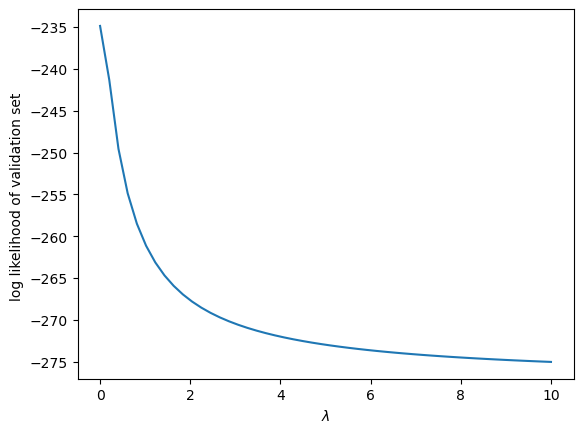
\includegraphics[width=10cm]{homework/homework_4/immages/q7_1.png}
\item 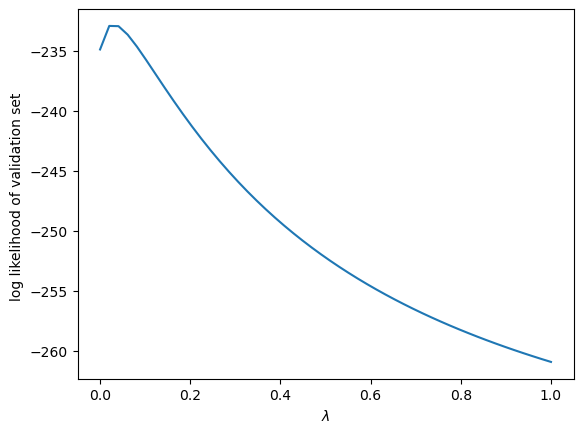
\includegraphics[width=10cm]{homework/homework_4/immages/q7_2.png}
\item 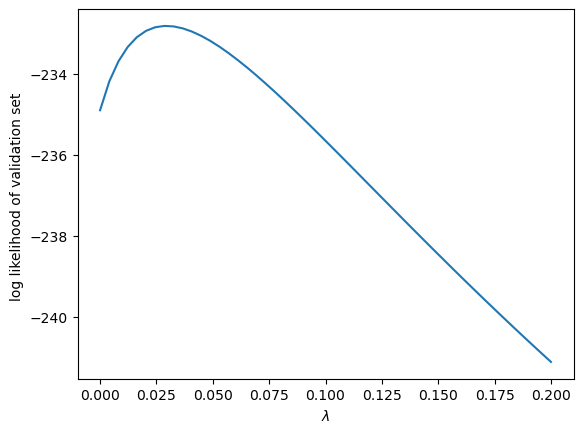
\includegraphics[width=10cm]{homework/homework_4/immages/q7_3.png}
\item i found optimal $\lambda =0.02857151428571429$
\end{itemize}
\item {[}Optional{]} 
It seems reasonable to interpret the prediction $f(x)=\phi(w^{T}x)=1/(1+e^{-w^{T}x})$
as the probability that $y=1$, for a randomly drawn pair $\left(x,y\right)$.
Since we only have a finite sample (and we are regularizing, which
will bias things a bit) there is a question of how well ``\href{https://en.wikipedia.org/wiki/Calibration_(statistics)}{calibrated}''
our predicted probabilities are. Roughly speaking, we say $f(x)$
is well calibrated if we look at all examples $\left(x,y\right)$
for which $f(x)\approx0.7$ and we find that close to $70\%$ of those
examples have $y=1$, as predicted... and then we repeat that for
all predicted probabilities in $\left(0,1\right)$. To see how well-calibrated
our predicted probabilities are, break the predictions on the validation
set into groups based on the predicted probability (you can play with
the size of the groups to get a result you think is informative).
For each group, examine the percentage of positive labels. You can
make a table or graph. Summarize the results. You may get some ideas
and references from \href{http://scikit-learn.org/stable/modules/calibration.html}{scikit-learn's discussion}.
\begin{itemize}
  \item \inputminted[firstline=174, lastline=191, breaklines=True]{python}{hw_4_code.py}
\item 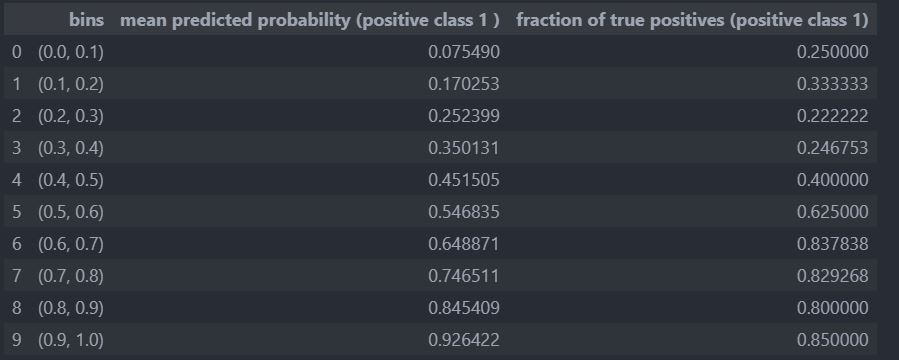
\includegraphics[width=10cm]{homework/homework_4/immages/question_8_1.JPG}
\item 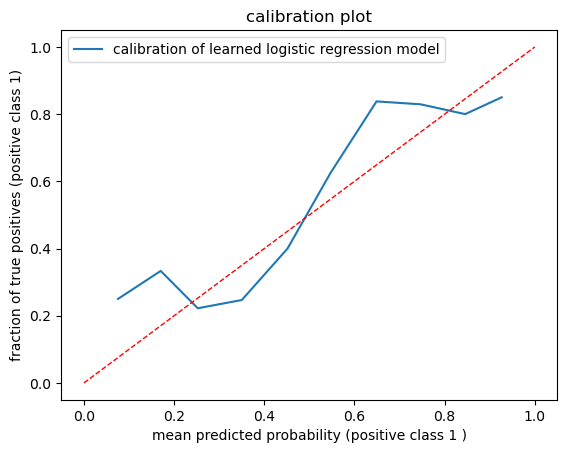
\includegraphics[width=10cm]{homework/homework_4/immages/q_8_2output.png}
\end{itemize}



\setcounter{saveenum}{\value{enumi}}
\end{enumerate}
\section{Coin Flipping with Partial Observability}
Consider flipping a biased coin where $p(z=H\mid \theta_1) = \theta_1$.
However, we cannot directly observe the result $z$.
Instead, someone reports the result to us,
which we denotey by $x$.
Further, there is a chance that the result is reported incorrectly \emph{if it's a head}.
Specifically, we have $p(x=H\mid z=H, \theta_2) = \theta_2$
and $p(x=T\mid z=T) = 1$.

\begin{enumerate}
  \setcounter{enumi}{\value{saveenum}}
\item Show that $p(x=H\mid \theta_1, \theta_2) = \theta_1 \theta_2$.
\begin{itemize}
    \color{blue}
    \item and assume that all $x_i$ are conditionally independent given z 
    \item we know that $z\in \{H,T\}$ so by the law of total probability $P(x=H|\theta_1,\theta_2)=P(x=H,z=H|\theta_1, \theta_2)+P(x=H,z=T|\theta_1, \theta_2)=P(z=H|\theta_1, \theta_2)P(X=h|z=H, \theta_1, \theta_2)+P(z=T|\theta_1, \theta_2)P(x=H|z=t,\theta_1, \theta_2)$
    \item we know that $P(x=T|Z=t)=1\Rightarrow P(X=H|z=T)=0$
    \item further we know z does not depends on $\theta_2$ so $P(z=h|\theta_1,\theta_2)=P(z=h|\theta_1)$
    \item and finally we know that $P(x=1|\theta_1, \theta_2, Z=H)=P(x=1|\theta_2, z=h)=\theta_2$ since the value of z is already set
    \item so thus we can see $ P(x=H|\theta_1,\theta_2)=\theta_1\theta_2$
\end{itemize}

\item Given a set of reported results $\mathcal{D}_r$ of size $N_r$, where the number of heads is $n_h$ and the number of tails is $n_t$, what is the likelihood of $\mathcal{D}_r$ as a function of $\theta_1$ and $\theta_2$.
\begin{itemize}
    \color{blue}
    \item here i am again assuming that $x_i$ is conditionally independent of $z_i$
    \item it is clear that $N_{r}=n_{h}+n_{t}$
    \item we can think of each reported coin flip $z_i$ as a Bernoulli with parameters ($\theta_1, \theta_2)$
    \item we know that the sum of conditionally independent Bernoulli is binomial 
    \item so we can say $\mathcal{L}(\theta_1, \theta_2, n_h)=\Pi_{i=1}^{n}P(x_i|\theta_1, \theta_2)= (P(x_i=h|\theta_1,\theta_2))^{n_h}(P(x_i=T|\theta_1,\theta_2))^{N_r-n_h}= (\theta_{1}\theta_{2})^{n_h}(P(x_i=T, z_i=H|\theta_1,\theta_2)+P(x_i=T, z_i=T|\theta_1,\theta_2))^{N_r-n_h}= (\theta_{1}\theta_{2})^{n_h}(P(z_i=H|\theat_1 ,\theta_2)P(x_i=T| z_i=H\theta_1,\theta_2)+P(z_i=T|\theta_1,\theta_2)P(x_i=T| z_i=T\theta_1,\theta_2))^{N_r-n_h}= (\theta_{1}\theta_{2})^{n_h}[(1-\theta_1)+\theta_1(1-\theta_2)]^{N_{r}-n_h}= (\theta_{1}\theta_{2})^{n_h}(1-\theta_1\theta_2)^{N_{R}-n_{h}}$
\end{itemize}


\item Can we estimate $\theta_1$ and $\theta_2$ using MLE? Explain your judgment.
\begin{itemize}
    \color{blue}
    \item i don't think we can estimate $\theta_1 , \theta_2$ it using mle
    \item we are only able to observe a binary outcome representing what we are told is the outcome but not the true outcome 
    \item so it is not possible for us to distinguish from our data set, what source of uncertainty comes from the coin flip $\theta_1$ or from if we will be told $\theta_2$
    \item i think we could maximise the likelihood of $\theta_1\theta_2$
\end{itemize}

\setcounter{saveenum}{\value{enumi}}
\end{enumerate}
\end{document}
